% Class X source questions transcribed from gadepall/cbse-papers, 2015/math/10.
% Source: https://github.com/gadepall/cbse-papers/blob/main/2015/math/10/cbse_2015_10.tex
\subsection{Section A}
\renewcommand{\theequation}{\theenumi}
\begin{enumerate}[label=\thesubsection.\arabic*,ref=\thesubsection.\theenumi]
\numberwithin{equation}{enumi}

\item If the quadratic equation $px^2-2\sqrt{5}px+15=0$ has two equal roots, find the value of $p$. \hfill (CBSE Class X, 2015, Q1)

\solution
For a quadratic equation $ax^2+bx+c=0$ to have equal roots, its discriminant must vanish:
\begin{align}
 b^2-4ac&=0.
\end{align}
Here $a=p$, $b=-2\sqrt{5}p$ and $c=15$. Therefore,
\begin{align}
 (-2\sqrt{5}p)^2-4(p)(15)&=0\\
 20p^2-60p&=0\\
 20p(p-3)&=0.
\end{align}
The algebraic possibilities are $p=0$ or $p=3$. However, $p=0$ removes the quadratic term and leaves $15=0$, which has no solution. Hence
\begin{align}
 \boxed{p=3}.
\end{align}

\item In Figure \ref{fig:class10-tower}, a tower $AB$ is $20\,\mathrm{m}$ high and $BC$, its shadow on the ground, is $20\sqrt{3}\,\mathrm{m}$ long. Find the Sun's altitude. \hfill (CBSE Class X, 2015, Q2)
\begin{figure}[H]
    \centering
    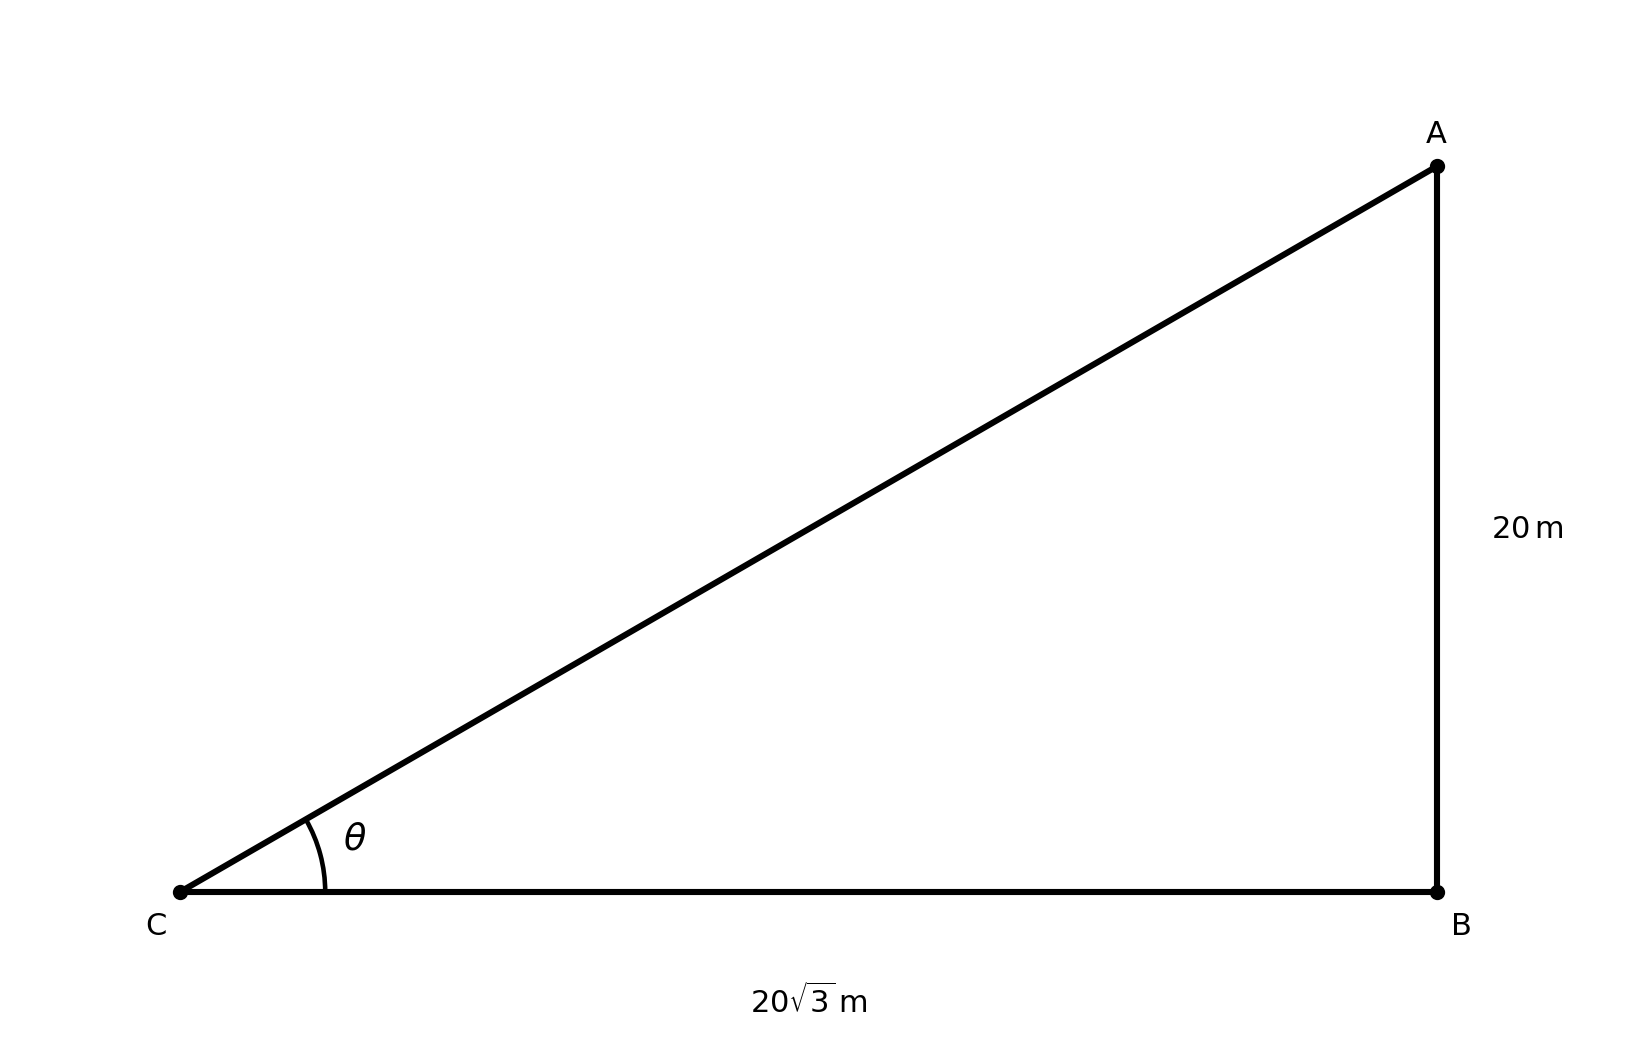
\includegraphics[width=0.83\linewidth]{figs/Tower.png}
    \caption{Tower and shadow; dimensions match the marking scheme.}
    \label{fig:class10-tower}
\end{figure}
\solution
The angle of elevation of the Sun is $\theta$. In right triangle $ABC$,
\begin{align}
 \tan\theta&=\frac{AB}{BC}=\frac{20}{20\sqrt{3}}=\frac{1}{\sqrt{3}},\
 \therefore\quad \boxed{\theta=30^\circ}.
\end{align}
The length $20\sqrt{3}\,\mathrm{m}$ is confirmed by the CBSE 2015 Class X marking scheme. The earlier source transcription omitted the radical and multiplier.

The figure was generated by the following Python script:
\begin{lstlisting}[frame=single,basicstyle=\rmfamily,escapeinside={(*@}{@*)}]
(*@\makebox[\dimexpr\linewidth-2\fboxsep-2\fboxrule\relax][c]{codes/Tower.py}@*)
\end{lstlisting}

\item Two different dice are tossed together. Find the probability that the product of the two numbers on the top of the dice is $6$. \hfill (CBSE Class X, 2015, Q3)

\solution
The two dice produce $6\times6=36$ equally likely ordered outcomes. The favourable ordered pairs are
\begin{align}
 (1,6),\ (6,1),\ (2,3),\ (3,2).
\end{align}
There are four favourable outcomes. Thus,
\begin{align}
 P(\text{product}=6)&=\frac{4}{36}=\boxed{\frac{1}{9}}.
\end{align}

\item In Figure \ref{fig:class10-chord-tangent}, $PQ$ is a chord of a circle with centre $O$ and $PT$ is a tangent. If $\angle QPT=60^\circ$, find $\angle PRQ$. \hfill (CBSE Class X, 2015, Q4)
\begin{figure}[H]
    \centering
    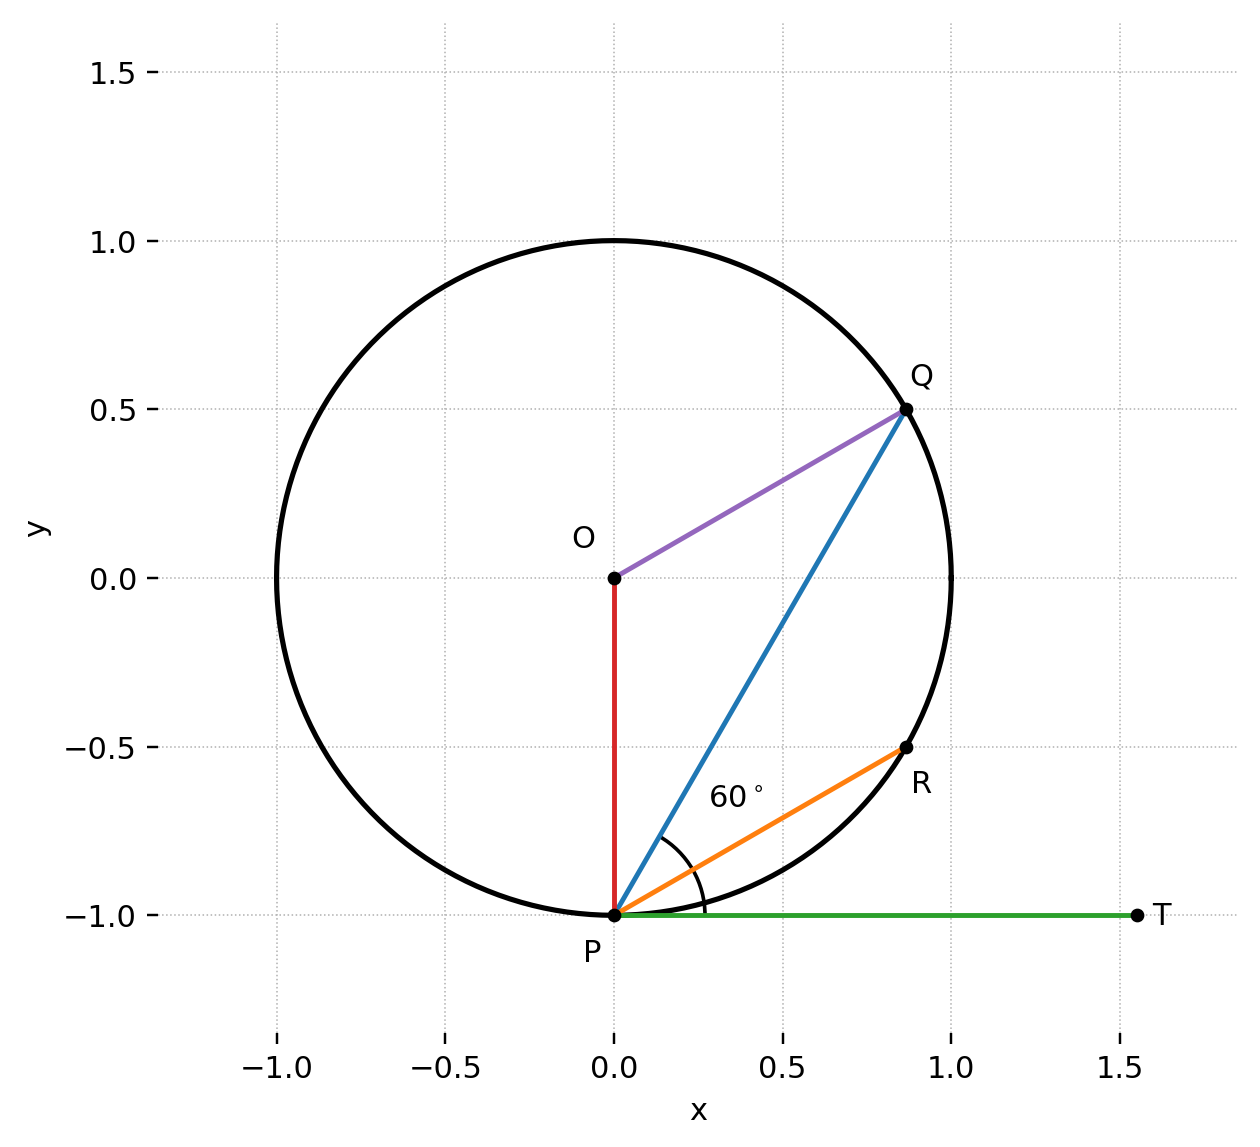
\includegraphics[width=0.66\linewidth]{figs/TangentChord.png}
    \caption{Chord and tangent configuration; drawn by Python.}
    \label{fig:class10-chord-tangent}
\end{figure}
\solution
Since a radius is perpendicular to the tangent at the point of contact, $\angle OPT=90^\circ$. Hence
\begin{align}
 \angle OPQ&=\angle OPT-\angle QPT=90^\circ-60^\circ=30^\circ.
\end{align}
As $OP=OQ$, triangle $OPQ$ is isosceles, so $\angle OQP=30^\circ$ and
\begin{align}
 \angle POQ&=180^\circ-30^\circ-30^\circ=120^\circ.
\end{align}
The point $R$ lies on the minor arc $PQ$ in the given figure. Therefore $\angle PRQ$ subtends the major arc $PQ$, whose measure is $360^\circ-120^\circ=240^\circ$. Thus
\begin{align}
 \angle PRQ&=\frac{240^\circ}{2}=\boxed{120^\circ}.
\end{align}

The figure was generated by the following Python script:
\begin{lstlisting}[frame=single,basicstyle=\rmfamily,escapeinside={(*@}{@*)}]
(*@\makebox[\dimexpr\linewidth-2\fboxsep-2\fboxrule\relax][c]{codes/TangentChord.py}@*)
\end{lstlisting}

\end{enumerate}

\subsection{Section B}
\begin{enumerate}[label=\thesubsection.\arabic*,ref=\thesubsection.\theenumi,start=5]
\numberwithin{equation}{enumi}

\item Two tangents $RQ$ and $RP$ are drawn from an external point $R$ to a circle with centre $O$. If $\angle PRQ=120^\circ$, prove that $OR=PR+RQ$. \hfill (CBSE Class X, 2015, Q5)
\begin{figure}[H]
    \centering
    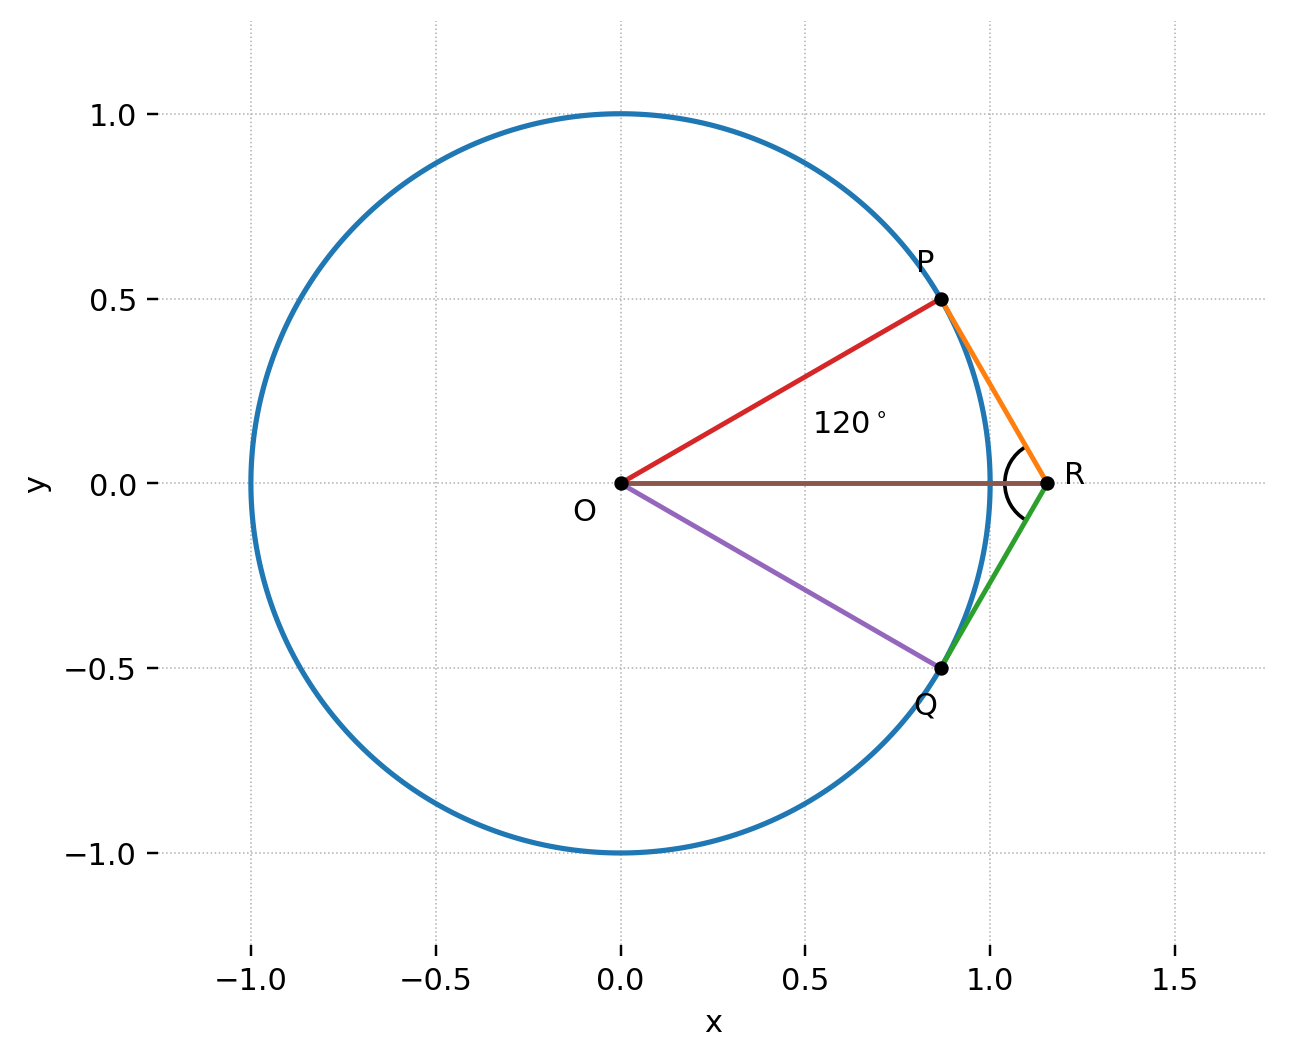
\includegraphics[width=0.64\linewidth]{figs/TwoTangents.png}
    \caption{Two tangents from an external point; drawn by Python.}
    \label{fig:class10-two-tangents}
\end{figure}
\solution
The radii to the points of contact are perpendicular to the tangents: $OP\perp PR$ and $OQ\perp QR$. The right triangles $\triangle OPR$ and $\triangle OQR$ are congruent by RHS, since $OP=OQ$ and $OR$ is common. Hence
\begin{align}
 PR=RQ,\qquad \angle PRO=\frac{1}{2}\angle PRQ=60^\circ.
\end{align}
In right triangle $OPR$,
\begin{align}
 \cos60^\circ&=\frac{PR}{OR}\\
 \frac{1}{2}&=\frac{PR}{OR}\\
 OR&=2PR.
\end{align}
Using $PR=RQ$ gives
\begin{align}
 \boxed{OR=PR+RQ}.
\end{align}

The figure was generated by the following Python script:
\begin{lstlisting}[frame=single,basicstyle=\rmfamily,escapeinside={(*@}{@*)}]
(*@\makebox[\dimexpr\linewidth-2\fboxsep-2\fboxrule\relax][c]{codes/TwoTangents.py}@*)
\end{lstlisting}
\end{enumerate}

\subsection{Batch audit}
Questions 1--5 in this batch are now based on the official 2015 Class X wording and figure configuration. The chapter ordering separates Question 5 into Section B, matching the official paper. Continue auditing the remaining questions against the official paper before submission.
